\documentclass[12pt]{article}

\usepackage{amsbsy}
\usepackage{amsmath}
\usepackage[dutch]{babel}
\usepackage{graphicx}
%\usepackage{gensymb}
\usepackage{float}

% Stop indent in nieuwe paragraaf
\setlength\parindent{0pt}

\begin{document}
    \title{\textbf{Practicum BB2: Brugschakelingen voor rekstrookjes} \\\small{Groep 2\_5}}
    \author{\textbf{Dries Van den Brande} \and Andreas Declerck \and Wassim Amghizar \and Joren Vermeersch}
    \date{\today}

    \maketitle

    \section{Doel van het practicum}

Svetlana.Verbruggen@vub.be

Emodulus bepalen
--> via rekstrookje, hoe werkt het?

Maat voor de stijheid van een materiaal. Sommige vervormen veel en andere weinig. Hoog weinig vervormen.

bpaling: door spanning = kracht / dwarsdoorsnele en wet van hooke

rekstrookje: kleine geleider, om de weerstand te bepalen. controle spanning op een materiaal.

Hoe werkt et: uitrek verandert de doorsnede --> verandering weerstan (pouillet)

basis eq: eq20
gausfactor: factor voor productiefouten

wat doen wij?
- Theoretisch berekenen van de gevoeligheid van beide types

opgave 2: schakeling maken, eerst paar dinge bereken (Theoretische waarde R en instellen)
welke combinatie mogen we niet maken?
bron niet meer ideaal --> 1.22
Interne weerstand verandert (hangt af van instelwaarde)

multimeter in gelijkstroon zetten

brug in evenwicht als Rmid = 0
dit door lineare interpolarisatie.

opgave 3: Emodulus bepalen

verslag:

Het doel van dit practicum wordt een brug van Wheatstone


\section{Doel}

In dit practicum wordt met behulp van de brug van Wheatstone
het elastisch gedrag van balkje met onbekende elasticitiet
onderzocht.


    \section{Theorie}

\subsection{Afleiding schuifkracht voor laminaire stroming en 
definitie van de viscositeit}

Als een voorwerp zich beweegt in een flu\"idum, dan verstoort het de snelheidsverdeling hiervan.
Vloeistofmoleculen die in onmiddelijk contact zijn met het voorwerp, krijgen door 
adhesiekrachten dezelfde snelheid, terwijl ver ervandaan het milieu niet verstoord wordt.\\

\begin{figure}[h]
    \centering
    \label{fig:snelheidsverdeling_laminair}
    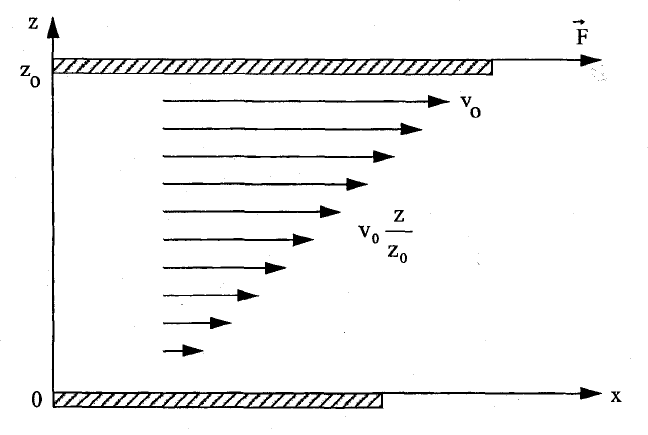
\includegraphics[width=0.7\textwidth]{img/figuur_1_theorie.png}
    \caption{Snelheidsverdeling in een viskeus midden tussen evenwijdige platen bij lage snelheden}
\end{figure}

Voor lage snelheden beweegt de vloeistof zich in lagen over elkaar. Dit heet \textbf{laminaire stroming}.
De laag $z = z_{0}$ heeft de snelheid $v_{0}$ de snelheid nul heeft. De snelheid van de 
vloeistoflagen daartussenin verandert lineair in functie van de hoogte z.
\\

$v = v_{0} \cdot \frac{z}{z_{0}}$ of $\frac{\delta v}{\delta z} = \frac{v_{0}}{z_{0}}$
\\

In het algemeen neemt de snelheid echter niet lineair toe met de dikte an de vloeistoflaag. 
De evenredigheidsconstante is ook afhankelijk van de aard van het flu\"idum, en wordt de
\textbf{viscositeitsco\"effici\"ent} genoemd. We bekomen de formule:
$$\frac{F_{W}}{S} = \eta \cdot \frac{dv}{dn}$$

Met
\\

$S=$ de oppervlakte van de vloeistoflagen

$n=$ de normaal loodrecht op dit oppervlak

$dv=$ de snelheidsverandering over de lengte

$dn=$ de normaal op S
\\

De \textbf{viscositeitsco\"effici\"ent} $\eta$ is dus de kracht per oppervlakte-eenheid nodig 
om snelheidsverschil van \'e\'en eenheid te handhaven tussen twee lagen vloeistof gelegen 
op een eenheidsfactor van elkaar.

\subsection{Laminaire stroming in een cilindervormige buis}

De wet van Hagen-Poiseuille geeft de snelheidsverdeling van de vloeistof 
in een horizontale cilindervormige buis bij stationaire, laminaire storming.
\\

$$v(r) = \frac{\pi(p_{1}-p_{2}) \cdot R^4}{4 \cdot L \cdot \eta}$$
\\
Het volumedebiet Q is het volume vloeistof dat per seconde door de buis stroomt.
Dit is te berekenen door die vergelijking over de doorsnede van de buis te integreren. 
Dit geeft: 
\\

$$\int_0^R2 \pi rdr \cdot v(r) = \frac{\pi(p_{1} - p_{2})\cdot R^4}{4 \cdot L \cdot \eta} $$
\\

Volgens de \textbf{wet van Poiseuille} is het debiet Q recht evenredig met het 
drukverschil $\delta p$ in het laminair regime. In een grafiek van Q in functie
van $\delta p$ geeft dit een rechte door de oorsprong; de richtingsco\"effici\"ent van de rechte is gelijk aan $\pi R^4 / 8\eta L$.
\\

\subsection{Overgang van laminair naar turbulent regime}

Als de snelheid echter te groot wordt, zal het laminair regime plaatsmaken voor een turbulent regime. 
Dit turbulente regime wordt gekenmerkt door wervelingen of draaikolkjes. Het hoogste
debiet waarbij de stroming nog juist stabiel laminair is, wordt het kritische debiet
$Q_{krit}$ genoemd.

\begin{figure}
    \caption{Grafiek overgang laminair naar turbulent regime}
    \label{fig:overgang_lam_turb}
    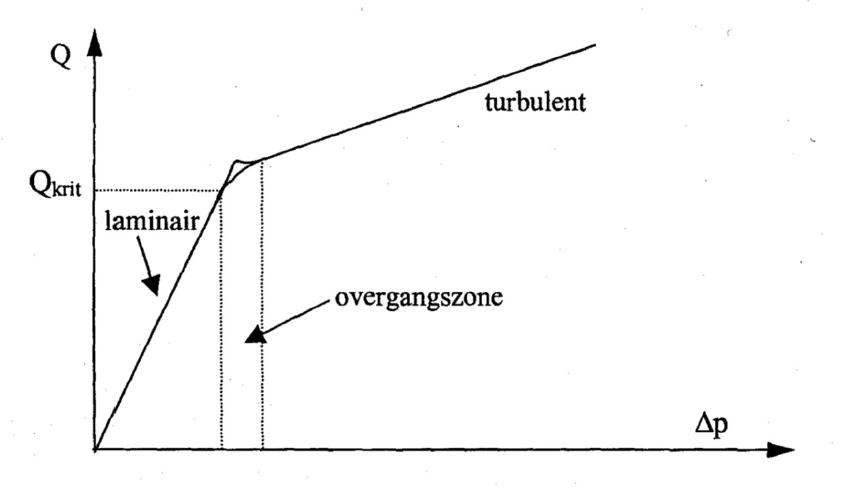
\includegraphics[width=0.7\textwidth]{img/figuur_3_theorie.png}
\end{figure}

Het is moeilijk om theoretisch te voorspellen bij welke stroomsnelheden laminaire
stroming zal overgaan in tubulente stroming. In dit kader speelt het 
\textbf{Reynoldgetal} een belangrijke rol.
\\

\subsection{Het Reynoldgetal}
De genormaliseerde gemiddelde stroomsnelheid $v/v_{0}$ wordt het Reynoldgetal genoemd:
\\

$$N_{R} = \frac{v \cdot \rho \cdot D}{\eta}$$
\\

Deze definitie geldt enkel voor een horizontale, cilindrische buis.
Voor andere systemen gelden andere definities.
\\

Het maximale Reynoldgetal waarbij de stroming nog juist stabiel is is ca. 2000.

    \section{Methode}

Door middel van een Hagen-Poiseuille opstelling (Figuur \ref{fig:hagen-pois}), kunnen we
enkele versimpelingen bekomen.

\begin{figure}[h]
    \caption{Hagen-Poiseuille opstelling}
    \includegraphics[width=\textwidth]{img/hagen_poiseuille.png}
    \label{fig:hagen-pois}
\end{figure}


    \section{Bepaling Gevoeligheid $Z$}
Als eerste opdracht bepalen we de gevoeligheid $Z$ van de brug in functie van alle 9 mogelijke combinaties
van de weerstanden $R_A$ en $zR_B$. We veronderstellen hiervoor deze waarden:
\begin{itemize}
    \item $U = 1 V$
    \item $R_X = 120 \Omega$
    \item $R_g = 100 \Omega$ voor de 2 eerste gevallen ($1000 \Omega$ voor de andere 2)
    \item $\Delta I = 10^{-7}$
\end{itemize}
Voor de Wheatstone brug type A gebruiken we de volgende formule:
\begin{equation}
    Z = U \cdot \frac{R_A}{R_A + R_B} \cdot \frac{1}{R_x + R_A + R_g + \frac{R_A}{R_B}\cdot R_g}
\end{equation}
Voor type A verwisselen we $R$ en $R_A$ van plaats in de formule:
\begin{equation}
    Z = U \cdot \frac{R}{R + R_B} \cdot \frac{1}{R_x + R + R_g + \frac{R}{R_B}\cdot R_g}
\end{equation}
Verder berekenen we tevens:
\begin{itemize}
    \item Evenwichtsvoorwaarde voor de instelbare weerstand $R$
    \item Kleinste verandering $\Delta R$ van $R$ om de brug in evenwicht te brengen
    \item Overeenstemmende kleinst mogelijk detecteerbare variatie $\Delta R_x$ van de te meten $R_x$ 
    \item Stroom door $R_A$ en $R_B$ bij evenwicht van de brug
\end{itemize}
We krijgen dus voor de 4 tabellen:
\begin{table}
    \centering
    \label{tab:Lamflow}
    \caption{Gemeten waarden in het turbulent regime}
    \begin{tabular}{| c | c | c | c | c | c | c | c | c |}
        \hline
                & $R_A [\Omega]$    & $R_B [\Omega]$    & $R [\Omega]$  & $Z [A]$               & $\Delta R [\Omega]$   & $\Delta R_x [\Omega]$ & $I_x [A]$                 & $I_B [A]$             \\ \hline
        1       & 10                & 10                & 120           & $1.52 \cdot 10^{-3}$  & $7.92 \cdot 10^{-3} $ & $7.92 \cdot 10^{-3} $ & $4.917 \cdot 10^{-3}$     & $5.00 \cdot 10^{-2} $ \\ \hline
        2       & 10                & 100               & 1200          & $3.79 \cdot 10^{-4}$  & $3.17 \cdot 10^{-2}$  & $3.17 \cdot 10^{-2}$  & $7.58 \cdot 10^{-4}$      & $9.09 \cdot 10^{-3}$  \\ \hline   
        3       & 10                & 1000              & 12000         & $4.29 \cdot 10^{-4}$  & $2.80 \cdot 10^{-4}$  & $2.80 \cdot 10^{-4}$  & $8.25 \cdot 10^{-4}$      & $9.90 \cdot 10^{-4}$  \\ \hline
        4       & 100               & 10                & 12            & $6.89 \cdot 10^{-4}$  & $3.79 \cdot 10^{-4}$  & $3.79 \cdot 10^{-4}$  & $3.79 \cdot 10^{-4}$      & $3.79 \cdot 10^{-4}$  \\ \hline
    \end{tabular}
\end{table}

$R = \frac{R_B}{R_A} \cdot R_X$
\\

$I_x = \frac{U}{R_{x} + R}$

$I_a = \frac{U}{R_{a} + R_{b}}

    \input{Wheatstone.tex}

    \section{Bepaling E modulus}

We meten op analoge wijze het rekstrookje.
Dit is bij $R_a$ en $R_b$ gelijk aan $10\Omega$ en 
men bekomt dan de waarden in tabel \ref{tab:rekstrookje}.
\\ \\
Men heeft hier gekozen voor een type $A$ opstelling omdat
er aan de nodige voorwaarde voor type $A$ werd voldaan.

Voorwaarde type $A$ opstelling:
$$ R_A > R en R_B > R_x of R_A < R en R_B < R_x $$

\begin{table}[h]
    \centering
    \caption{Meetresultaten rekstrookje}
    \label{tab:rekstrookje}

    \begin{tabular}{| c | c | c | c | c |}
        \hline
        Kracht [N] & $R_{min} [\Omega]$& $R_{max} [\Omega]$& $I_{min}$ [mA] & $I_{max}$ [mA] \\ \hline
        0,981      & 130               & 120               & -0,041    & 0,003 \\ \hline
        1,962      & 130               & 120               &-0,047     & 0,003 \\ \hline
        2,943      & 130               & 120               &-0,04      & 0,004 \\ \hline
        3,924      & 130               & 120               &-0,04      & 0,004 \\ \hline
        4,905      & 130               & 120               &-0,039     & 0,004 \\ \hline
        5,886      & 130               & 120               &-0,039     & 0,004 \\ \hline
        6,867      & 130               & 120               &-0,038     & 0,005 \\ \hline
    \end{tabular}
\end{table}

\begin{figure}[h]
    \centering
    \caption{Lineaire interpolatie}
    \label{fig:lin_interpol_e}
    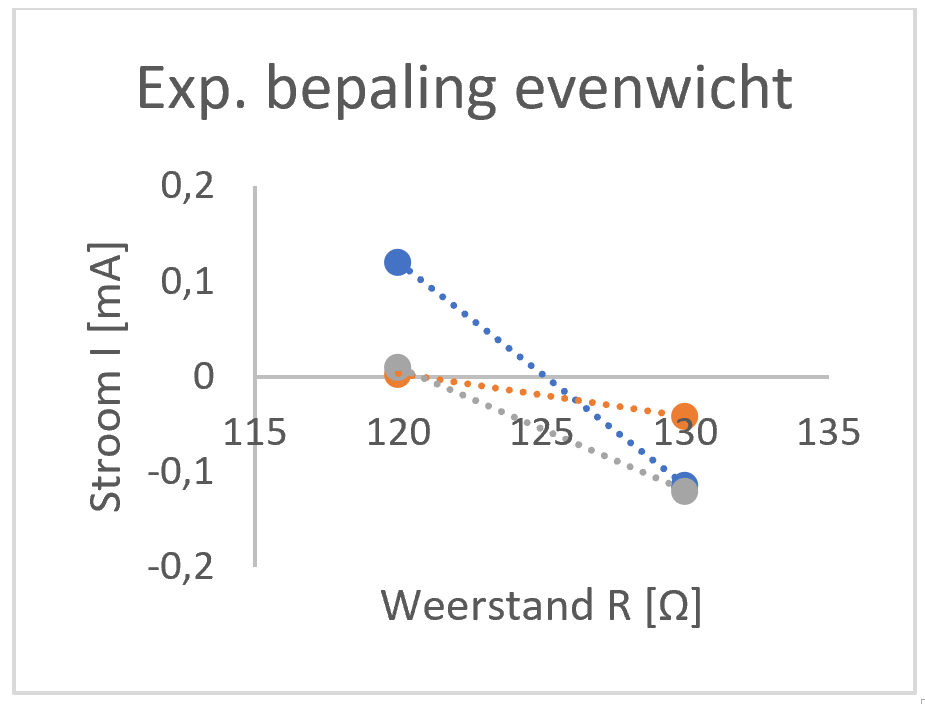
\includegraphics[width=0.7\textwidth]{img/tweede.png}
\end{figure}

Na interpolatie [\ref{fig:lin_interpol_e}] volgens volgende formule:

\begin{equation}
    R = R_{min} - \frac{\Delta R}{\Delta I} \cdot I_{min}
\end{equation}


bekomt men R. Met deze waarde wordt het mogelijk om $R_{x}$ te
berekenen via een schaalfactor 1 bepaald door $R_{a}$ en $R_{b}$.
\\

$\Delta R_{x}$ wordt dan weer bepaald door het verschil met de
nominale waarde van het rekstrookje (waarde van de weerstand
bij evenwicht, ongeveer $120\Omega$).
\\ \\
Men bekomt de waarden uit tabel \ref{tab:interpol_rekstrookje}

\begin{table}[h]
    \centering
    \caption{Interpolatie rekstrookje}
    \label{tab:interpol_rekstrookje}
    \begin{tabular}{| c | c | c | c |}
        \hline
        R [$\Omega$]    & Rx [$\Omega$] & $\Delta R_{x}$    & $\frac{\Delta R_{x}}{R_{x}}$ \\ \hline
        120,682         & 120,682       & 0,682             & 0,005650 \\ \hline
        120,600         & 120,600       & 0,600             & 0,004975 \\ \hline
        120,909         & 120,909       & 0,909             & 0,007519 \\ \hline
        120,909         & 120,909       & 0,909             & 0,007519 \\ \hline
        120,930         & 120,930       & 0,930             & 0,007692 \\ \hline
        120,930         & 120,930       & 0,930             & 0,007692 \\ \hline
        121,163         & 121,163       & 1,163             & 0,009597 \\ \hline
    \end{tabular}
\end{table}

Nu kan men een lineaire regressie uitvoeren met als x-waarden
de krachten uitgeoefend op het balkje en als y-waarden
$\frac{\Delta R_{x}}{R_{x}}$.

\begin{figure}[h]
    \centering
    \caption{Lineaire regressie $E$}
    \label{fig:lin_reg_E}
    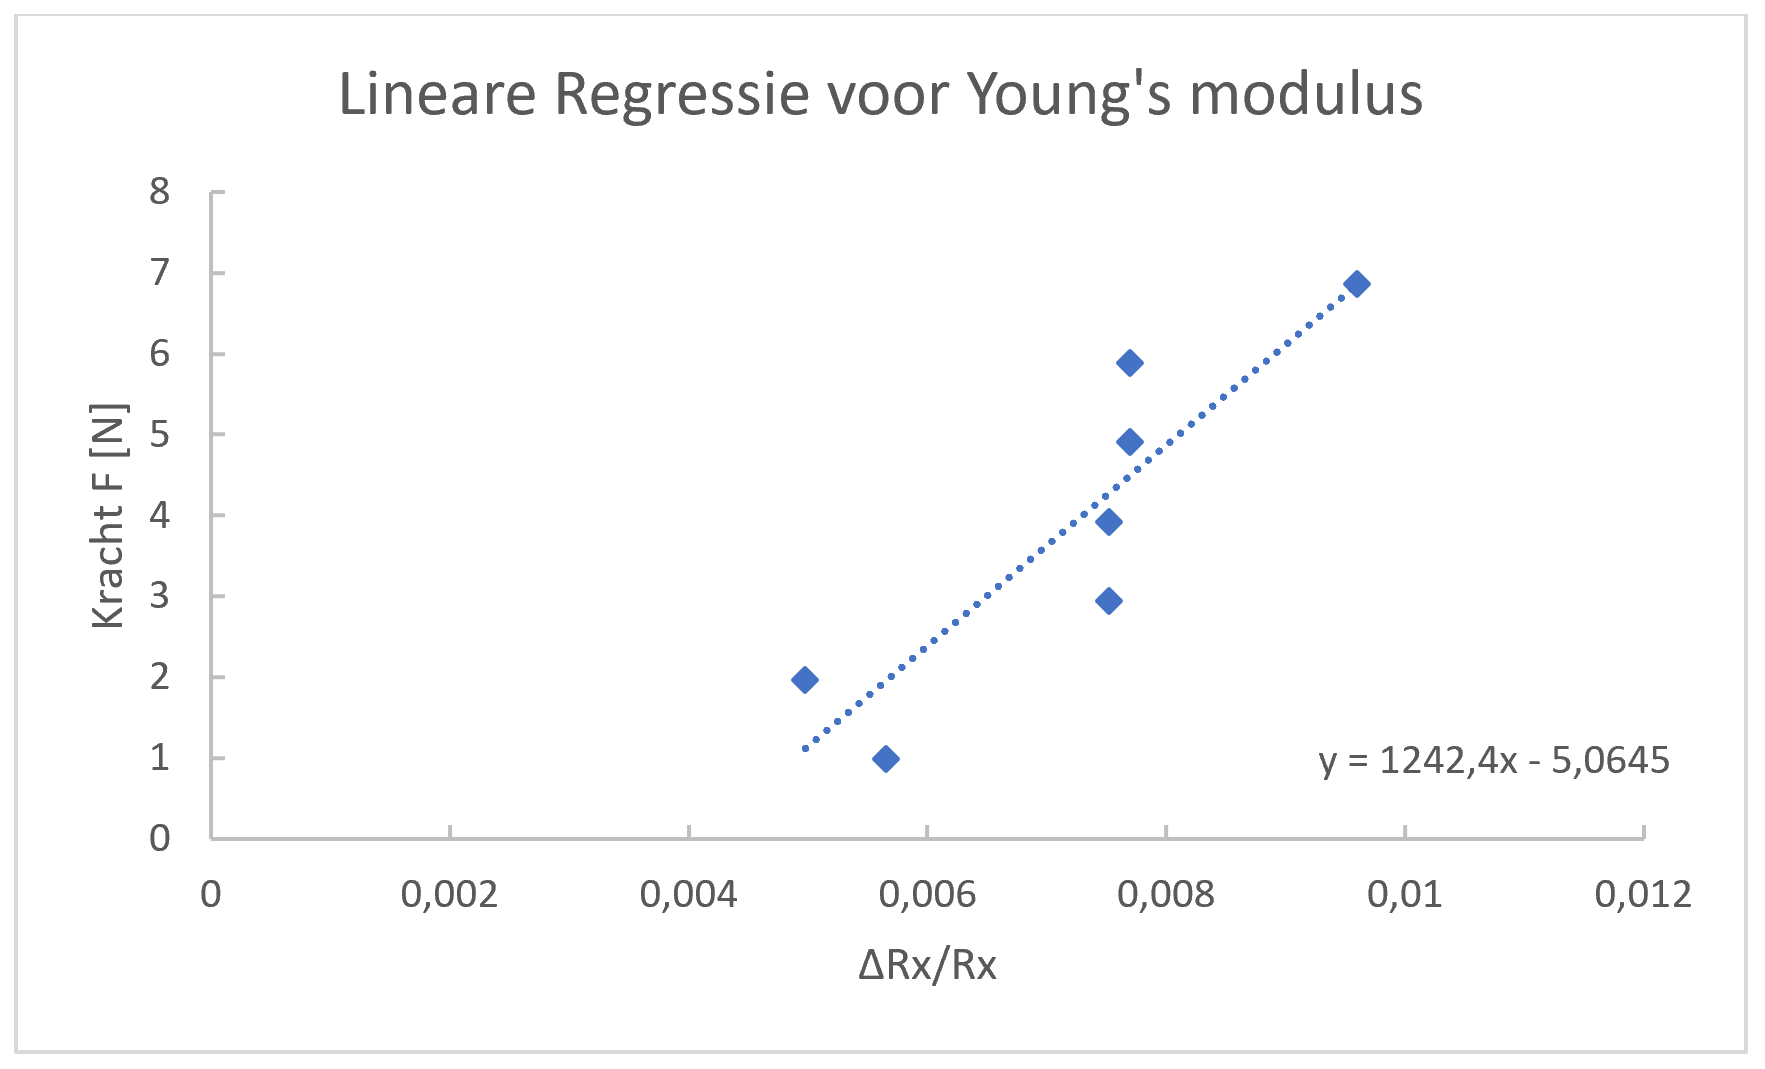
\includegraphics[width=0.7\textwidth]{img/grafiek.png}
\end{figure}

Met de lineaire regressie [\ref{fig:lin_reg_E}] functie in excel kan men nu de
richtingsco\"effici\"ent bepalen. Deze zal van volgende vorm
zijn:

\begin{equation}
    m = \frac{3}{2} \cdot \frac{K_1 \cdot L}{E \cdot b \cdot d^2}
\end{equation}

Na enige omvorming krijgt men een formule voor $E$:

\begin{equation}
    E = \frac{3}{2} \cdot \frac{K_1 \cdot L}{z \cdot b \cdot d^2}
\end{equation}

Samen met volgende fysische eigenschappen van het balkje:

\begin{table}[h]
    \centering
    \caption{Fysische eigenschappen balkje}
    \label{tab:fys_eig_balkje}
    \begin{tabular}{| c | c | c |}
        \hline
            & Waarde& Fout \\ \hline
        K1  & 2,110 & 0,01 \\ \hline
        L   & 0,250 & 0,00 \\ \hline
        b   & 0,020 & 0,00 \\ \hline
        d   & 0,005 & 0,00 \\ \hline
    \end{tabular}
\end{table}

Kan men nu $E$ en de fout hierop berekenen:

\begin{equation}
    E = 9,964E+09 \pm 4,7E+07
\end{equation}

\subsection{Bespreking resultaten}

Hoewel men hier een waarde uikomt ziet men dat de proeven
niet al te accuraat werden uitgevoerd. Dit kan liggen aan
de materiaalpech die men ervaarde tijdens het practicum. Ook
tijdstekort bezorgde extra druk waardoor er
onnauwkeurigheden gemakkelijk konden insluipen.



    \section{Foutenanalyse}
\subsection{Rechtstreekse grootheden}
\subsection{Systematische fouten}
Bij opgave 3 werd de stroom rechtstreeks opgemeten met behulp van een digitale multimeter.
De opgegeven reading en digits bedraagt 1\% rdg + 1 dig.
De instrumentale fout wordt bepaald door 1\% van de afgelezen waarde te nemen en op te tellen met 0,1.


    \section{Conclusie}
De berekende waarden zijn accuraat bepaald.
De schatting van het Reynoldgetal zou nog kunnen verbeterd worden door meer datapunten 
te meten rond het overgangspunt van laminair naar turbulent regime.

    \bibliographystyle{plain}
\bibliography{../ref}
\end{document}